\documentclass[11pt,a4paper]{article}

\usepackage[margin=2.5cm]{geometry}
\usepackage[T1]{fontenc}
\usepackage[utf8]{inputenc}
\usepackage{lmodern}
\usepackage{microtype}
\usepackage{graphicx}
\usepackage{placeins}
\usepackage{booktabs}
\usepackage[hidelinks]{hyperref}
\usepackage{xurl}
\usepackage[nameinlink]{cleveref}

\graphicspath{{figures/}}

\title{Urban Outfinders\\[0.3em]\large Part 4: RAG, User Interface and Web Analytics}
\author{Marc Mallol\and Èric Dürr\and Oriol Pont}
\date{Information Retrieval and Web Analytics, 2026}

\begin{document}
\maketitle

\section{Introduction}

In this final part we turn the search engine of Parts~1 to~3 into a web application. Users type a query in a search box, get the products ranked by any of the Part~3 rankers (the custom score by default), read a short recommendation written by a LLM from those results, and can afterwards open a page with all the details of a product. Meanwhile, the app records how it is used, and a dashboard shows these statistics.

The code is at \url{https://github.com/uripont/IRWA-2026-u213930-u213920-u215106}, tag \texttt{IRWA-2026-part-4}. The search function is in \path{search.py}, the LLM summaries in \path{rag.py}, the usage data in \path{analytics.py} and the Flask app in \path{web/}, all inside the \path{fashion_search} package. The README explains how to start the app (\texttt{uv run python -m fashion\_search.web}) and \path{notebooks/part_4.ipynb} produces the numbers and examples in this report.

\section{Search engine for the web}
\subsection{Search function}

The web app only talks to the engine through one function, \texttt{Searcher.search(query, method, page)}. It receives the text exactly as the user typed it, the ranking method (\texttt{custom}, \texttt{bm25}, \texttt{tfidf} or \texttt{word2vec}) and the page number, and returns one page of 20 results together with what the results page needs to explain them: the total number of products found, the query terms after pre-processing, whether the matching had to be "relaxed" (see below) and the time it took in ms. Each result already holds the fields the page shows (title, description, brand, category, prices, discount, rating, stock, the link to the original store and the first image), so the templates never touch the catalogue directly. An unknown method falls back to the default instead of failing (since anyone can edit the URL).

The \texttt{Searcher} loads the catalogue and builds the inverted index once, when the app starts (about 2 seconds), and then keeps every ranker of Part~3 ready. The text processing, AND matching and scoring are the same functions as in the notebooks of Parts~2 and~3, so the app ranks exactly as we evaluated. The default is the custom score, because Part~3 found it kept the quality of BM25 (AP 0.988 against 0.990) while almost removing out-of-stock products from the top 20 and raising their average rating, which is what matters most to someone shopping.

\subsection{Optimisations for a real use case}

The biggest limit we found in Part~3 was AND matching itself: as soon as one query word appears in no product, the user gets an empty page. This happens a lot with real queries (for example: a typo, a brand the catalogue does not sell,...). So, to keep a good user experience, when no product contains every term, the search keeps the products that contain the largest number of distinct query terms, ranks them with the chosen method using only the terms they can match, and tells the user how many words were matched and which words no result contains. \Cref{tab:relaxed} shows three such queries. For \emph{nike running shoes men} the user gets the 37 running shoes for men, and the page explains that none of them is a Nike product. For \emph{men leather jacket puma} there are 79 products with three of the four words, and the first ones are men's leather jackets of other brands. Relaxed matching does not correct typos, though. For \emph{blue jeens} the user gets every blue product plus the only product whose description has the same typo, which is a pair of jeans and goes to the top since the rare term weighs more. A spelling correction step would handle these queries better, and we leave it as future work, outside of the scope of this project. AND matching is still used whenever it returns something, so the five test queries of Part~2 get exactly the same results as before.

\begin{table}[ht]
  \centering
  \begin{tabular}{lrrl}
    \toprule
    Query & Results & Terms matched & Missing from every result \\
    \midrule
    blue jeens & 7,697 & 1 of 2 & none \\
    nike running shoes men & 37 & 3 of 4 & nike \\
    men leather jacket puma & 79 & 3 of 4 & none \\
    \bottomrule
  \end{tabular}
  \caption{Queries with no product containing every term, answered with relaxed matching. ``None'' means that each missing word is found in some of the results.}
  \label{tab:relaxed}
\end{table}

The second change is about speed. Ranking a query scores every candidate, but the results page only shows 20 of them, and the same query is asked (again) for the next pages and for the LLM summary. So the full ranking of each query and method is computed once and kept in a cache of the last 256 queries, and the next page of a query takes about 1~ms. Word2Vec also needed its own fix, since training its model took about 23 seconds every time the engine started. Now the model is saved to disk after the first training and loaded in about 0.3 seconds afterwards (it is trained again only if the catalogue changes). \Cref{tab:speed} shows the time of a search without the cache. Every method answers the test queries in a few milliseconds, and the slowest case is \emph{blue jeens}, where relaxed matching returns more than 7,000 products to score.

\begin{table}[ht]
  \centering
  \begin{tabular}{lrrrr}
    \toprule
    & Custom score & BM25 & TF-IDF & Word2Vec \\
    \midrule
    Median over the 8 queries (ms) & 4.0 & 2.1 & 2.1 & 2.3 \\
    Slowest query, \emph{blue jeens} (ms) & 38.5 & 9.9 & 10.9 & 25.9 \\
    \bottomrule
  \end{tabular}
  \caption{Time of one search with an empty cache (median of 5 runs, notebook section 1.2). A cached page takes about 1~ms.}
  \label{tab:speed}
\end{table}

\subsection{Application structure}

As the statement asks, the app is built with Flask and runs on Flask's own development server (in the same way Python and the notebooks were given from the start of the project). It lives in \path{web/__init__.py}, which uses an application factory (\texttt{create\_app}) that creates one \texttt{Searcher} and one \texttt{AnalyticsStore} and attaches them to the app, so the routes share them and a test or the notebook can pass its own. It has five routes:

\begin{itemize}
  \item \texttt{/}, the search page.
  \item \texttt{/search?q=\ldots\&method=\ldots\&page=\ldots}, the results page. It uses GET, so every results page has its own URL (that therefore could be bookmarked or shared), and the back button of the browser works as expected.
  \item \texttt{/summary}, which returns the LLM summary of a query as JSON. The results page asks for it with JavaScript once it has loaded, so the user sees the products right away instead of waiting for the LLM. If the API refuses or fails (for example when the rate limit of the free tier is reached), the box shows a short message instead of the summary, and without an API key it is simply left out. Answers are cached, so repeating a search does not call the API again.
  \item \texttt{/product/<pid>}, the page of one product. Links from the results page add the query and the rank of the product, so the click can be logged with them.
  \item \texttt{/dashboard}, the analytics dashboard (\cref{sec:analytics}).
\end{itemize}

Each visitor gets a random session identifier stored in a signed cookie, and after every page request the app logs the request, plus the query or the click when there is one, in the analytics store. Static files are not logged, so the data only describes what users actually do. The templates share a base layout with the search box in the header, so a new search can be started from any page.

\section{User interface}
\label{sec:ui}
\subsection{Search page}

The search page (\cref{fig:search}) is a single search box in the middle of the page, with a menu to choose the ranking method and a button. For this report, we kept it as simple as possible (\cref{app:restyle} shows a version closer to a modern e-commerce site, on the same Flask stack), since most users will just type and press enter, and the menu defaults to the custom score so nobody has to choose. The line below the box explains how matching works (every word, or the closest matches otherwise), so the results never come as a surprise, and the five test queries of Part~2 are offered as examples that can be clicked.

\begin{figure}[ht]
  \centering
  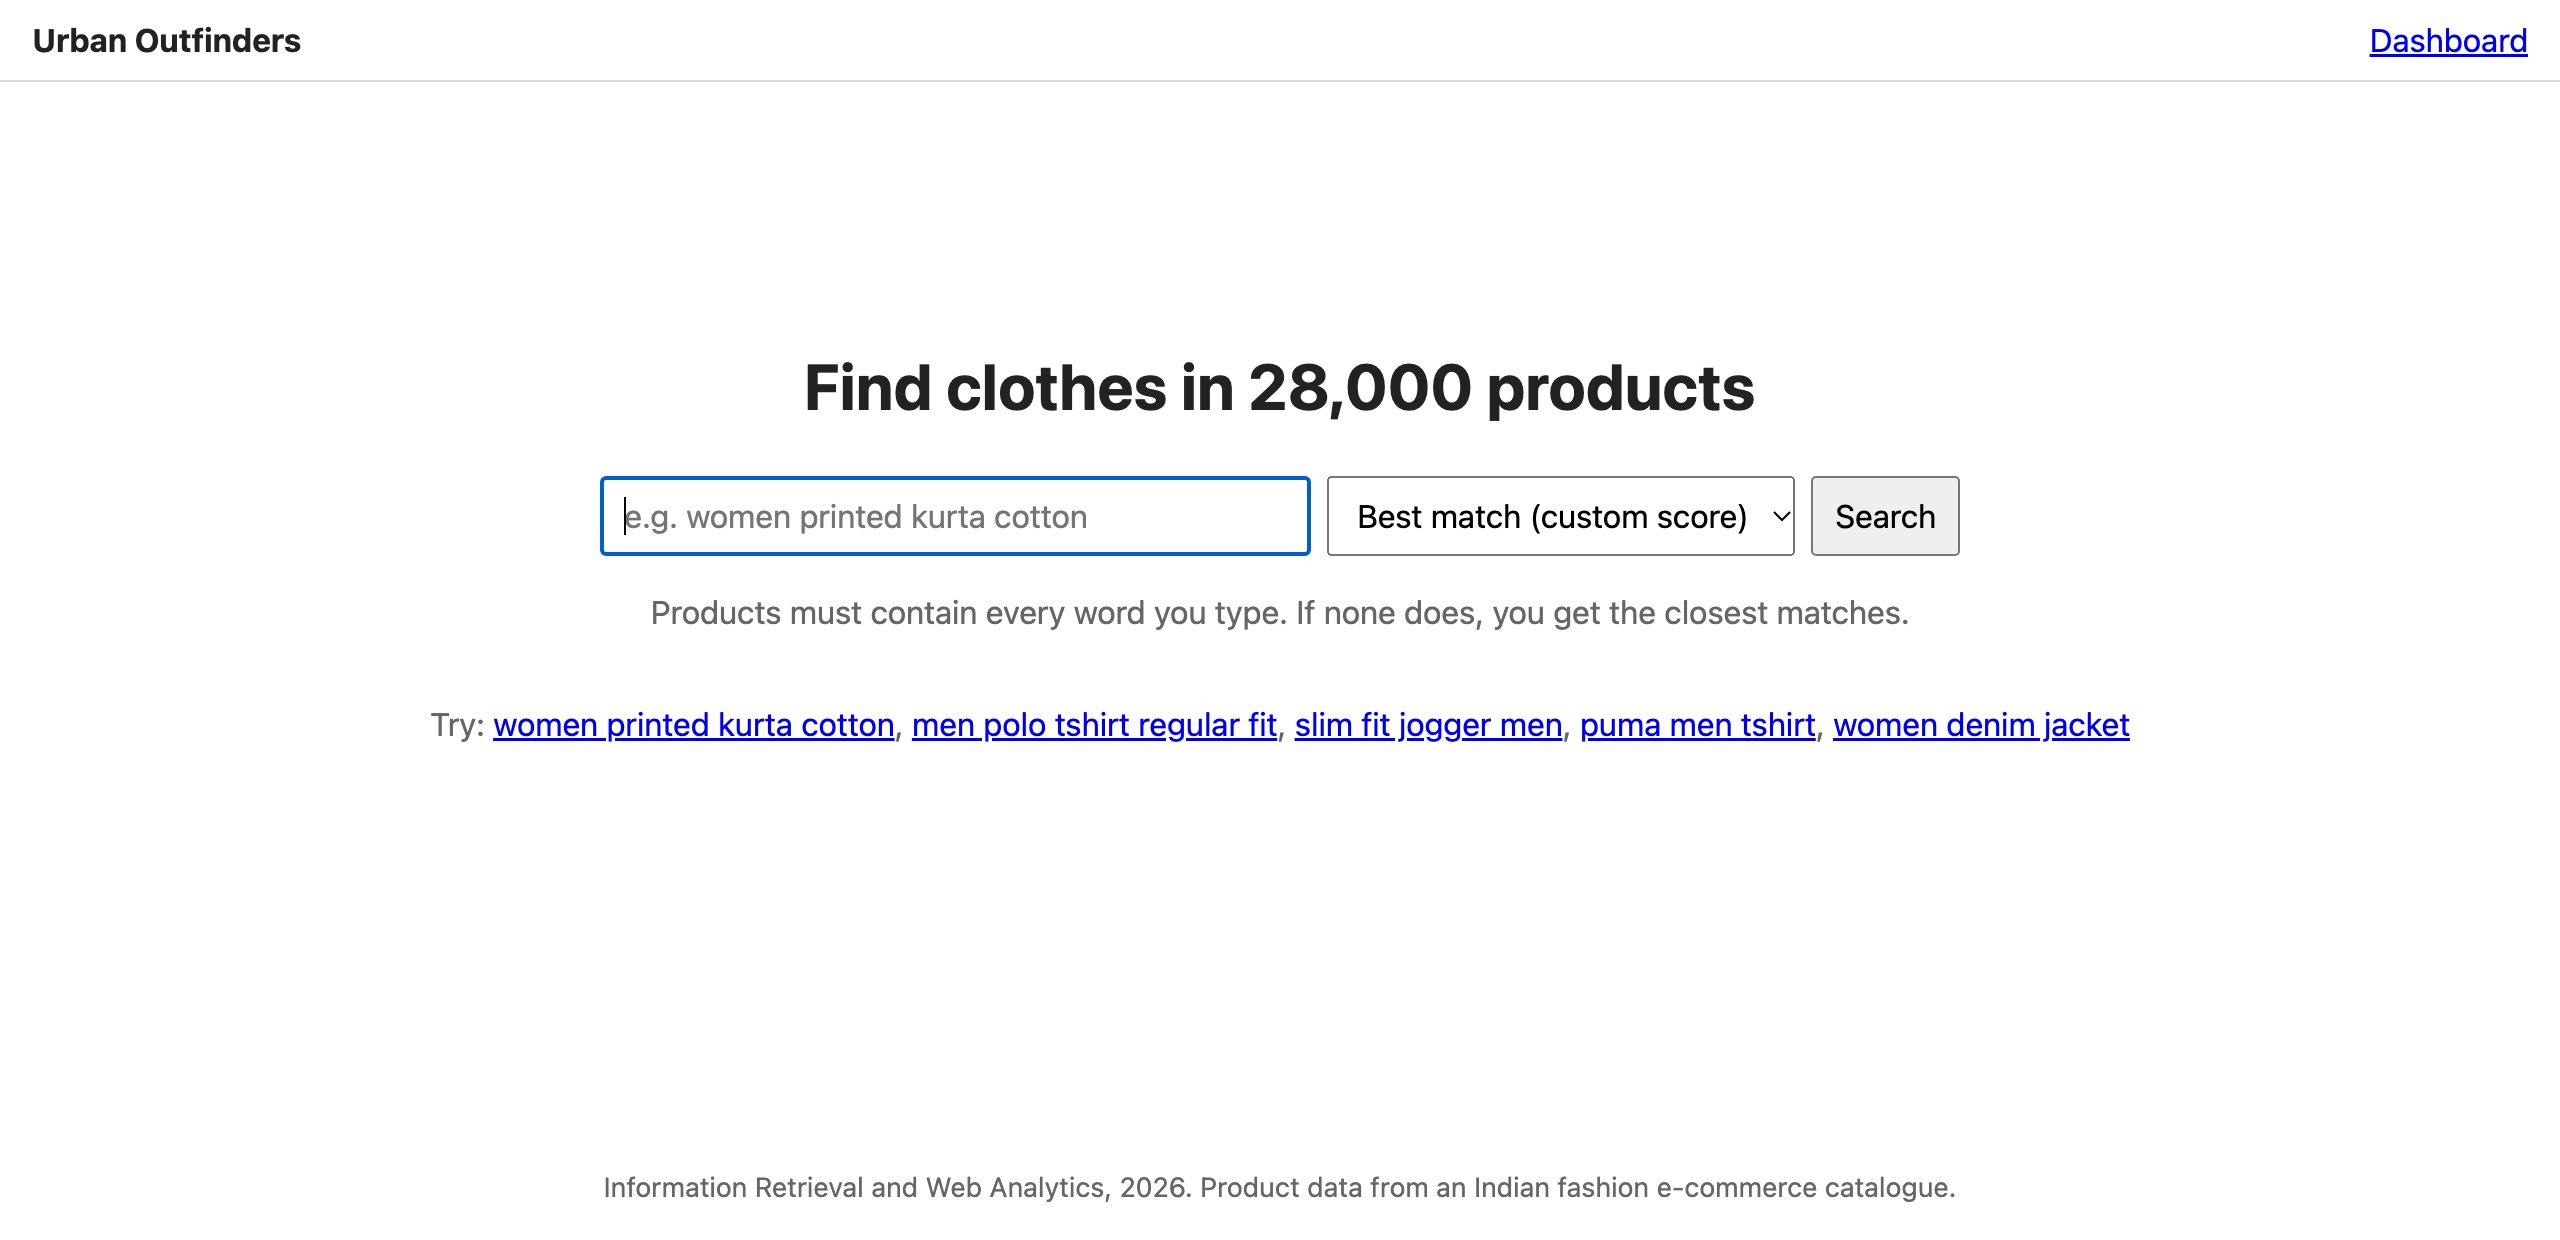
\includegraphics[width=\textwidth]{search.png}
  \caption{Search page.}
  \label{fig:search}
\end{figure}

\subsection{Results page}

The results page (\cref{fig:results}) shows the products in the order of the ranking, 20 per page with links to the previous and next pages. Above them, it shows how many products were found and how long the search took, a menu to rank the same query with another method, and the LLM summary when it is available. Each result has the fields the statement asks for (title, description, selling price, discount, average rating and a link to the product in the original store) and three more that we found useful when trying the app ourselves: a picture of the product (in fashion people often decide by the picture first), the brand and category, and the original price crossed out next to the selling price, so the discount is easy to read. Products that are out of stock get a label, since the user cannot buy them. The title and the picture lead to the product page, and long descriptions are shortened (the whole text is on the product page).

\begin{figure}[ht]
  \centering
  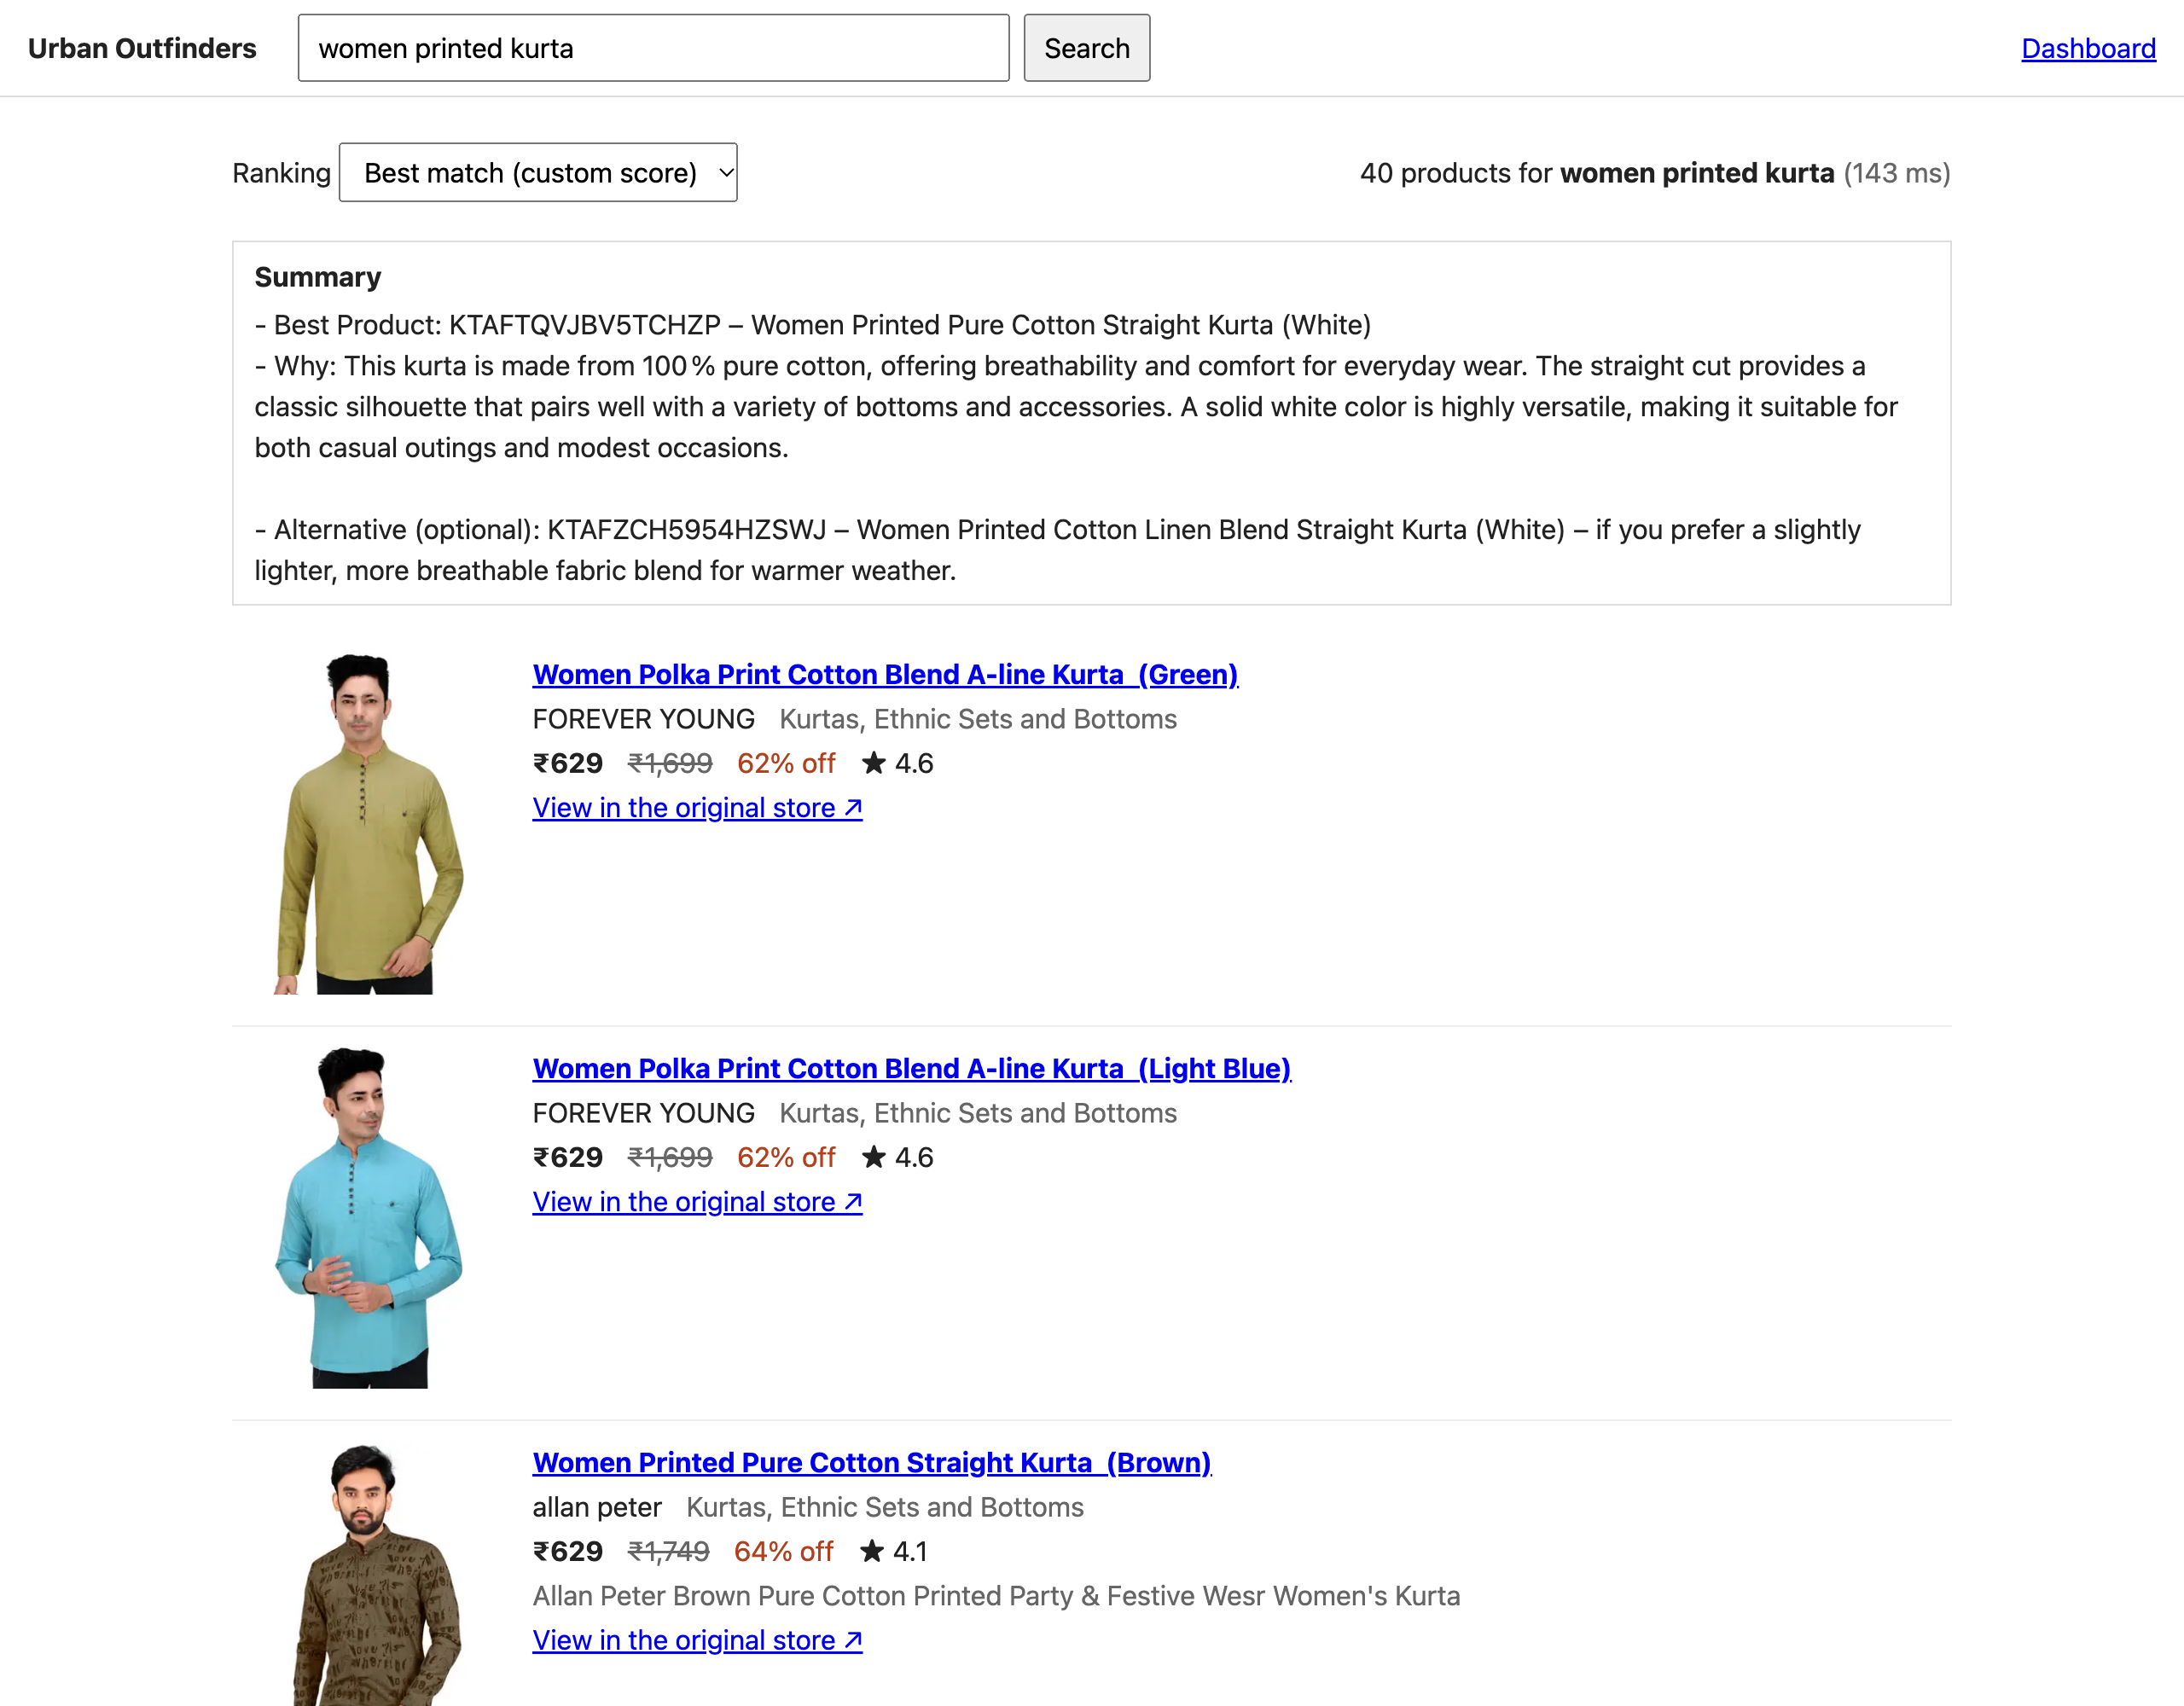
\includegraphics[width=\textwidth]{results.png}
  \caption{Results page for \emph{women printed kurta}, ranked by the custom score.}
  \label{fig:results}
\end{figure}

When relaxed matching was needed, a notice above the results says so (\cref{fig:relaxed}). We think this is important because otherwise the user would believe that every result contains every word, and would not understand why a query asking for Puma shows jackets of another brand.

\begin{figure}[ht]
  \centering
  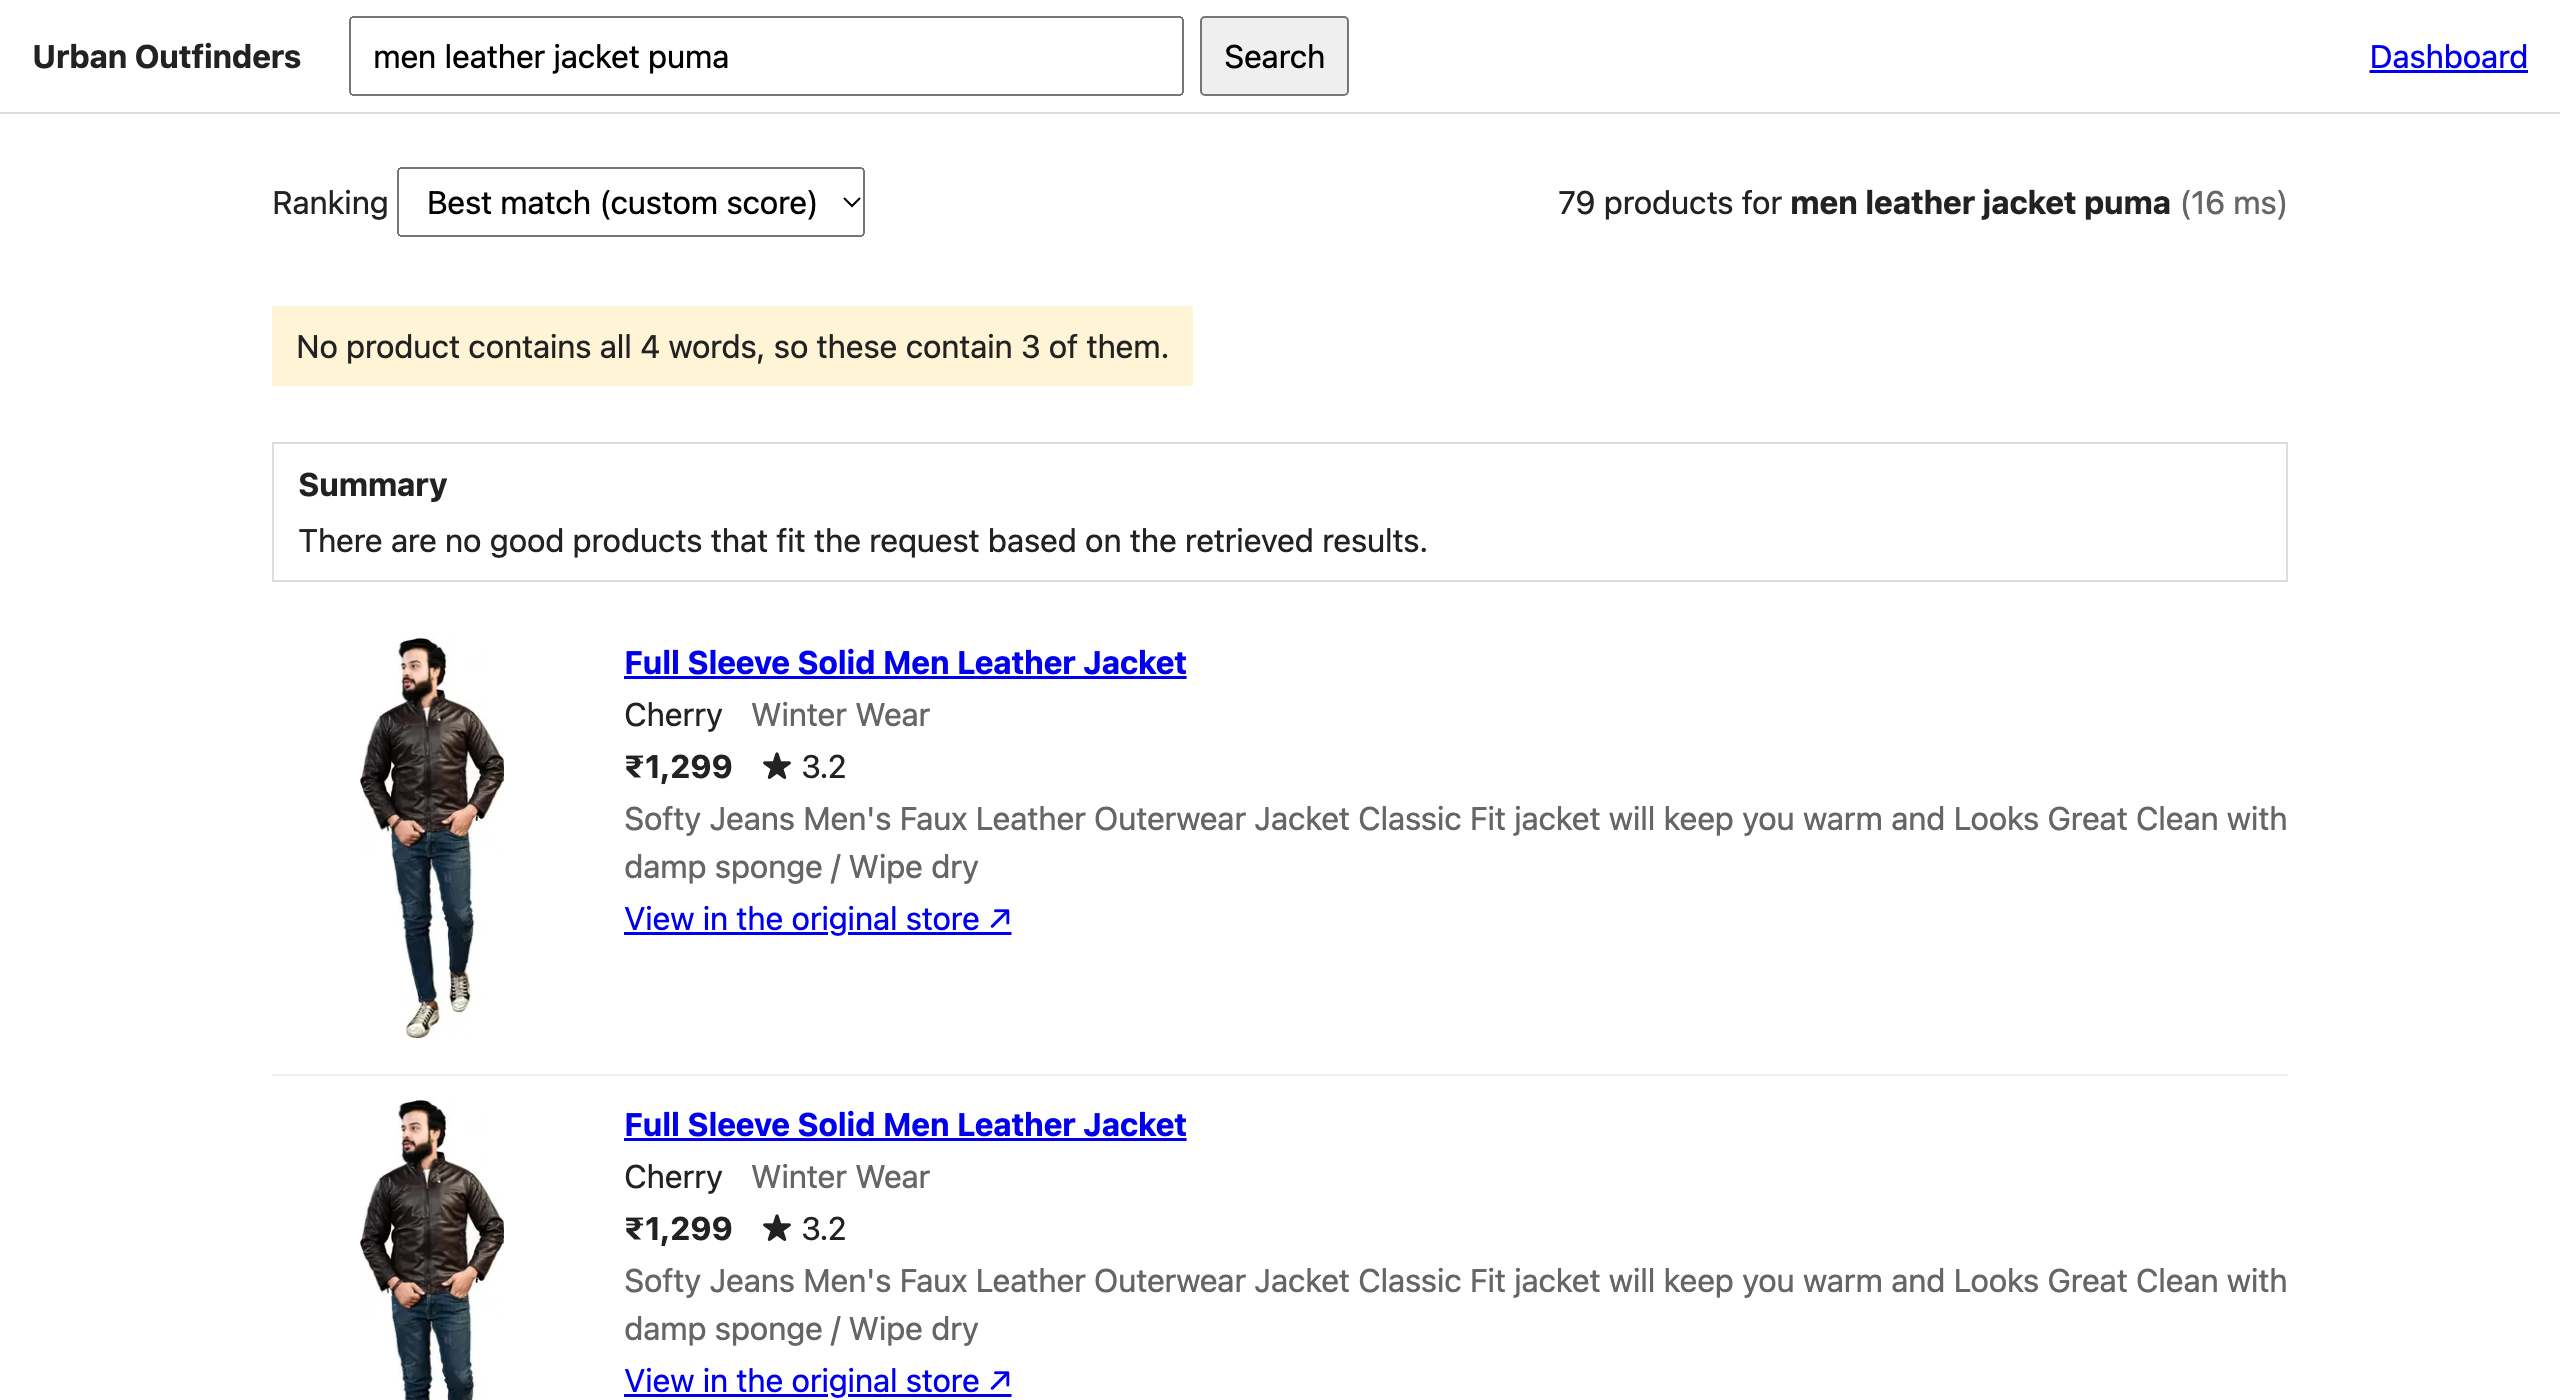
\includegraphics[width=\textwidth]{relaxed.png}
  \caption{Results page when no product contains every query term.}
  \label{fig:relaxed}
\end{figure}

\subsection{Product page}

The product page (\cref{fig:product}) shows everything the catalogue has about a product: all its pictures (the dataset links small thumbnails, so the app asks the image server for a bigger version of the same picture), the title, brand, stock, prices and rating, the full description, and a table with the product details (fabric, fit, sleeve, colour, and so on, which change from one product to another), the category and subcategory, the seller and the product ID. A button opens the product in the original store, and when the user came from a results page, a link takes them back to the same results.

\begin{figure}[ht]
  \centering
  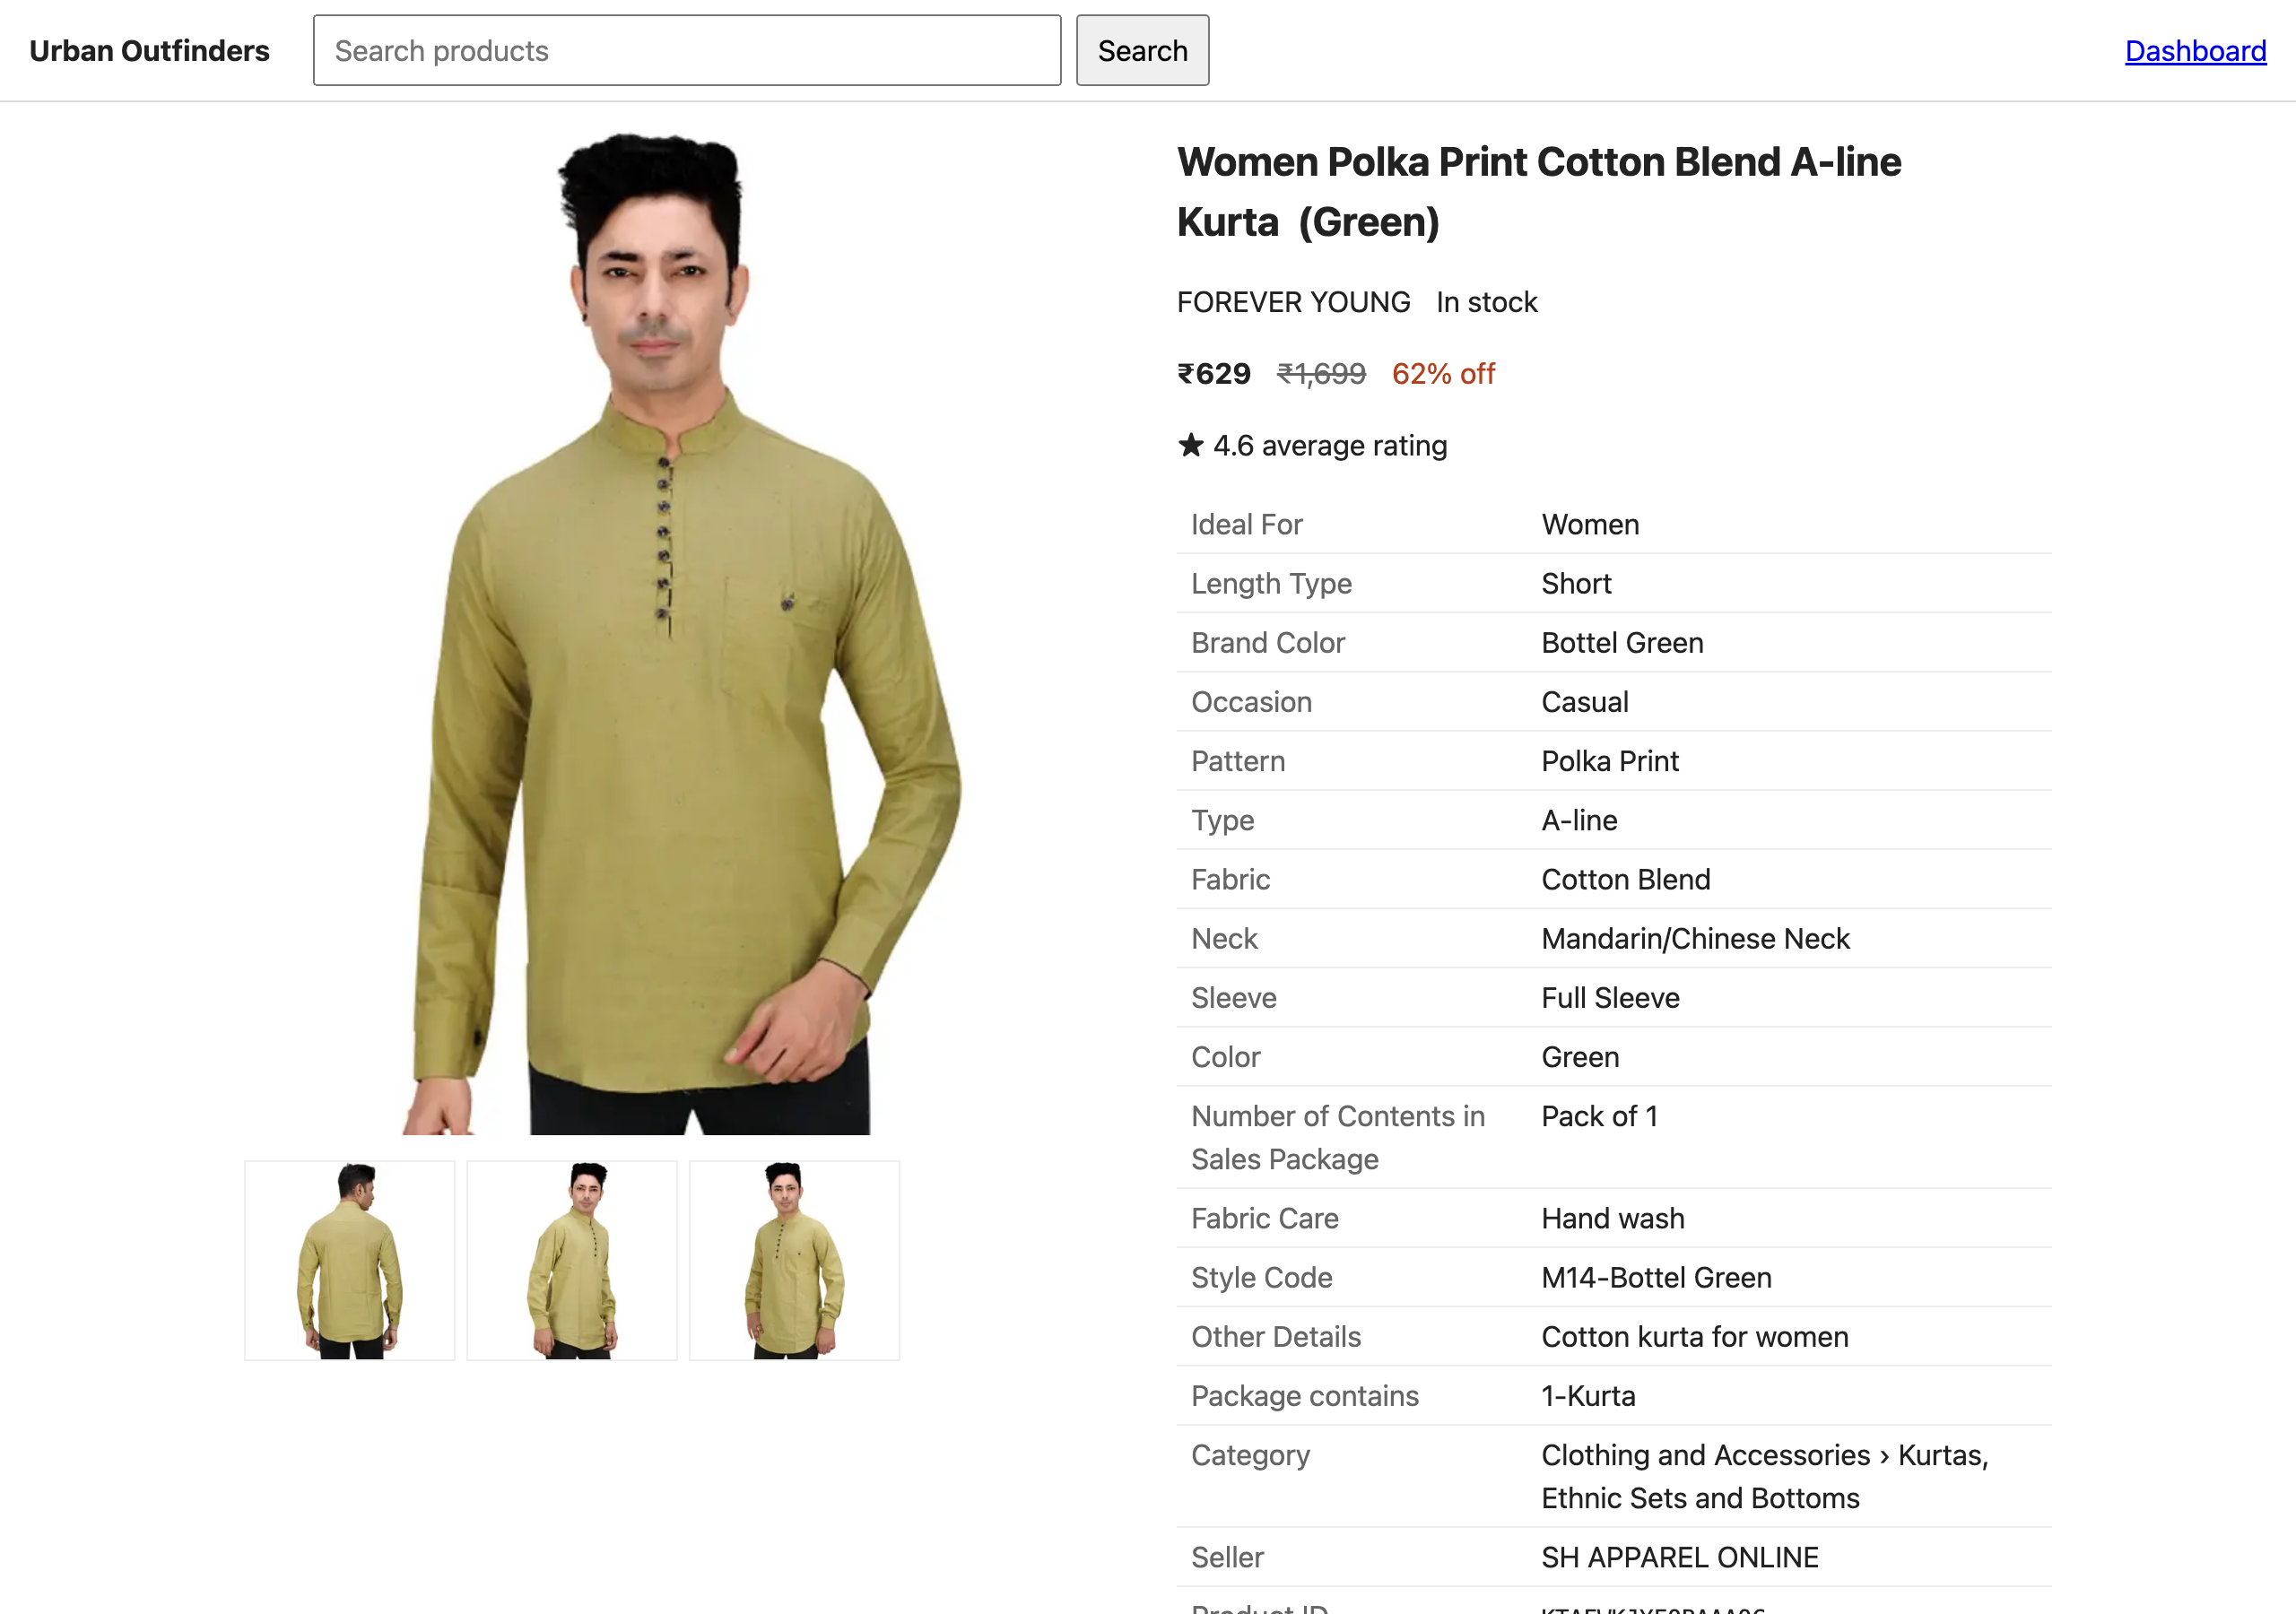
\includegraphics[width=\textwidth]{product.png}
  \caption{Product page (cropped).}
  \label{fig:product}
\end{figure}

\FloatBarrier
\section{Retrieval-augmented generation}
\subsection{Baseline and its weaknesses}
% TODO(RAG): the template's baseline and its weaknesses, with examples.

\subsection{Improvements}
% TODO(RAG): two or three improvements, with pros and cons.

\subsection{Baseline against improved}
% TODO(RAG): examples on the same queries, including one where no product fits.

\section{Web analytics}
\label{sec:analytics}
\subsection{Data collection}
% TODO(analytics): what is collected and why.

\subsection{Data model}
% TODO(analytics): the star schema.

\subsection{Dashboard}
% TODO(analytics): indicators and graphs, each explained.

\section{Conclusion}
% TODO: what Part 4 achieves and its main limitations.

\section*{Use of AI tools}
% As in Part 3: which tools we used and for what.

The visual overhaul of \cref{app:restyle} was mostly driven by AI (Claude, through Claude Code). Once we had chosen the inspiration for it, the assistant wrote a first draft of the templates and the style sheet. It worked, but it still did not look like a real shop, so we kept critiquing it page by page (on a computer and on a phone screen) and asking for changes, over three more rounds, until we were satisfied with the visual result. Each round is a separate commit in the repository, from the first draft to the final version.

\clearpage
\appendix
\section{Visual overhaul}
\label{app:restyle}

Once the app worked, we gave it a look closer to a modern fashion store, inspired by the Urban Outfitters website (only its layout and typography, none of its logo, pictures or text). The search engine, routes and data are the ones of \cref{sec:ui}, and the app is still plain Flask templates with one CSS file and a few lines of JavaScript, so the stack the statement asks for is unchanged. All of it lives in the templates and the style sheet, so the search, the LLM summaries and the analytics work exactly as described in the rest of the report.

What we took from that kind of site is mostly an attitude: pictures first, a lot of white space, black type with large titles, and nothing on the page that only makes sense to the people who built the engine. The header (logo, search box and link to the dashboard) is the same on every page and does not move between them, so the user always knows where to search again. \Cref{fig:restyle-home,fig:restyle-results,fig:restyle-product} show it on a computer, and the end of this appendix lists the changes in detail and shows it on a phone.

\begin{figure}[h!]
  \centering
  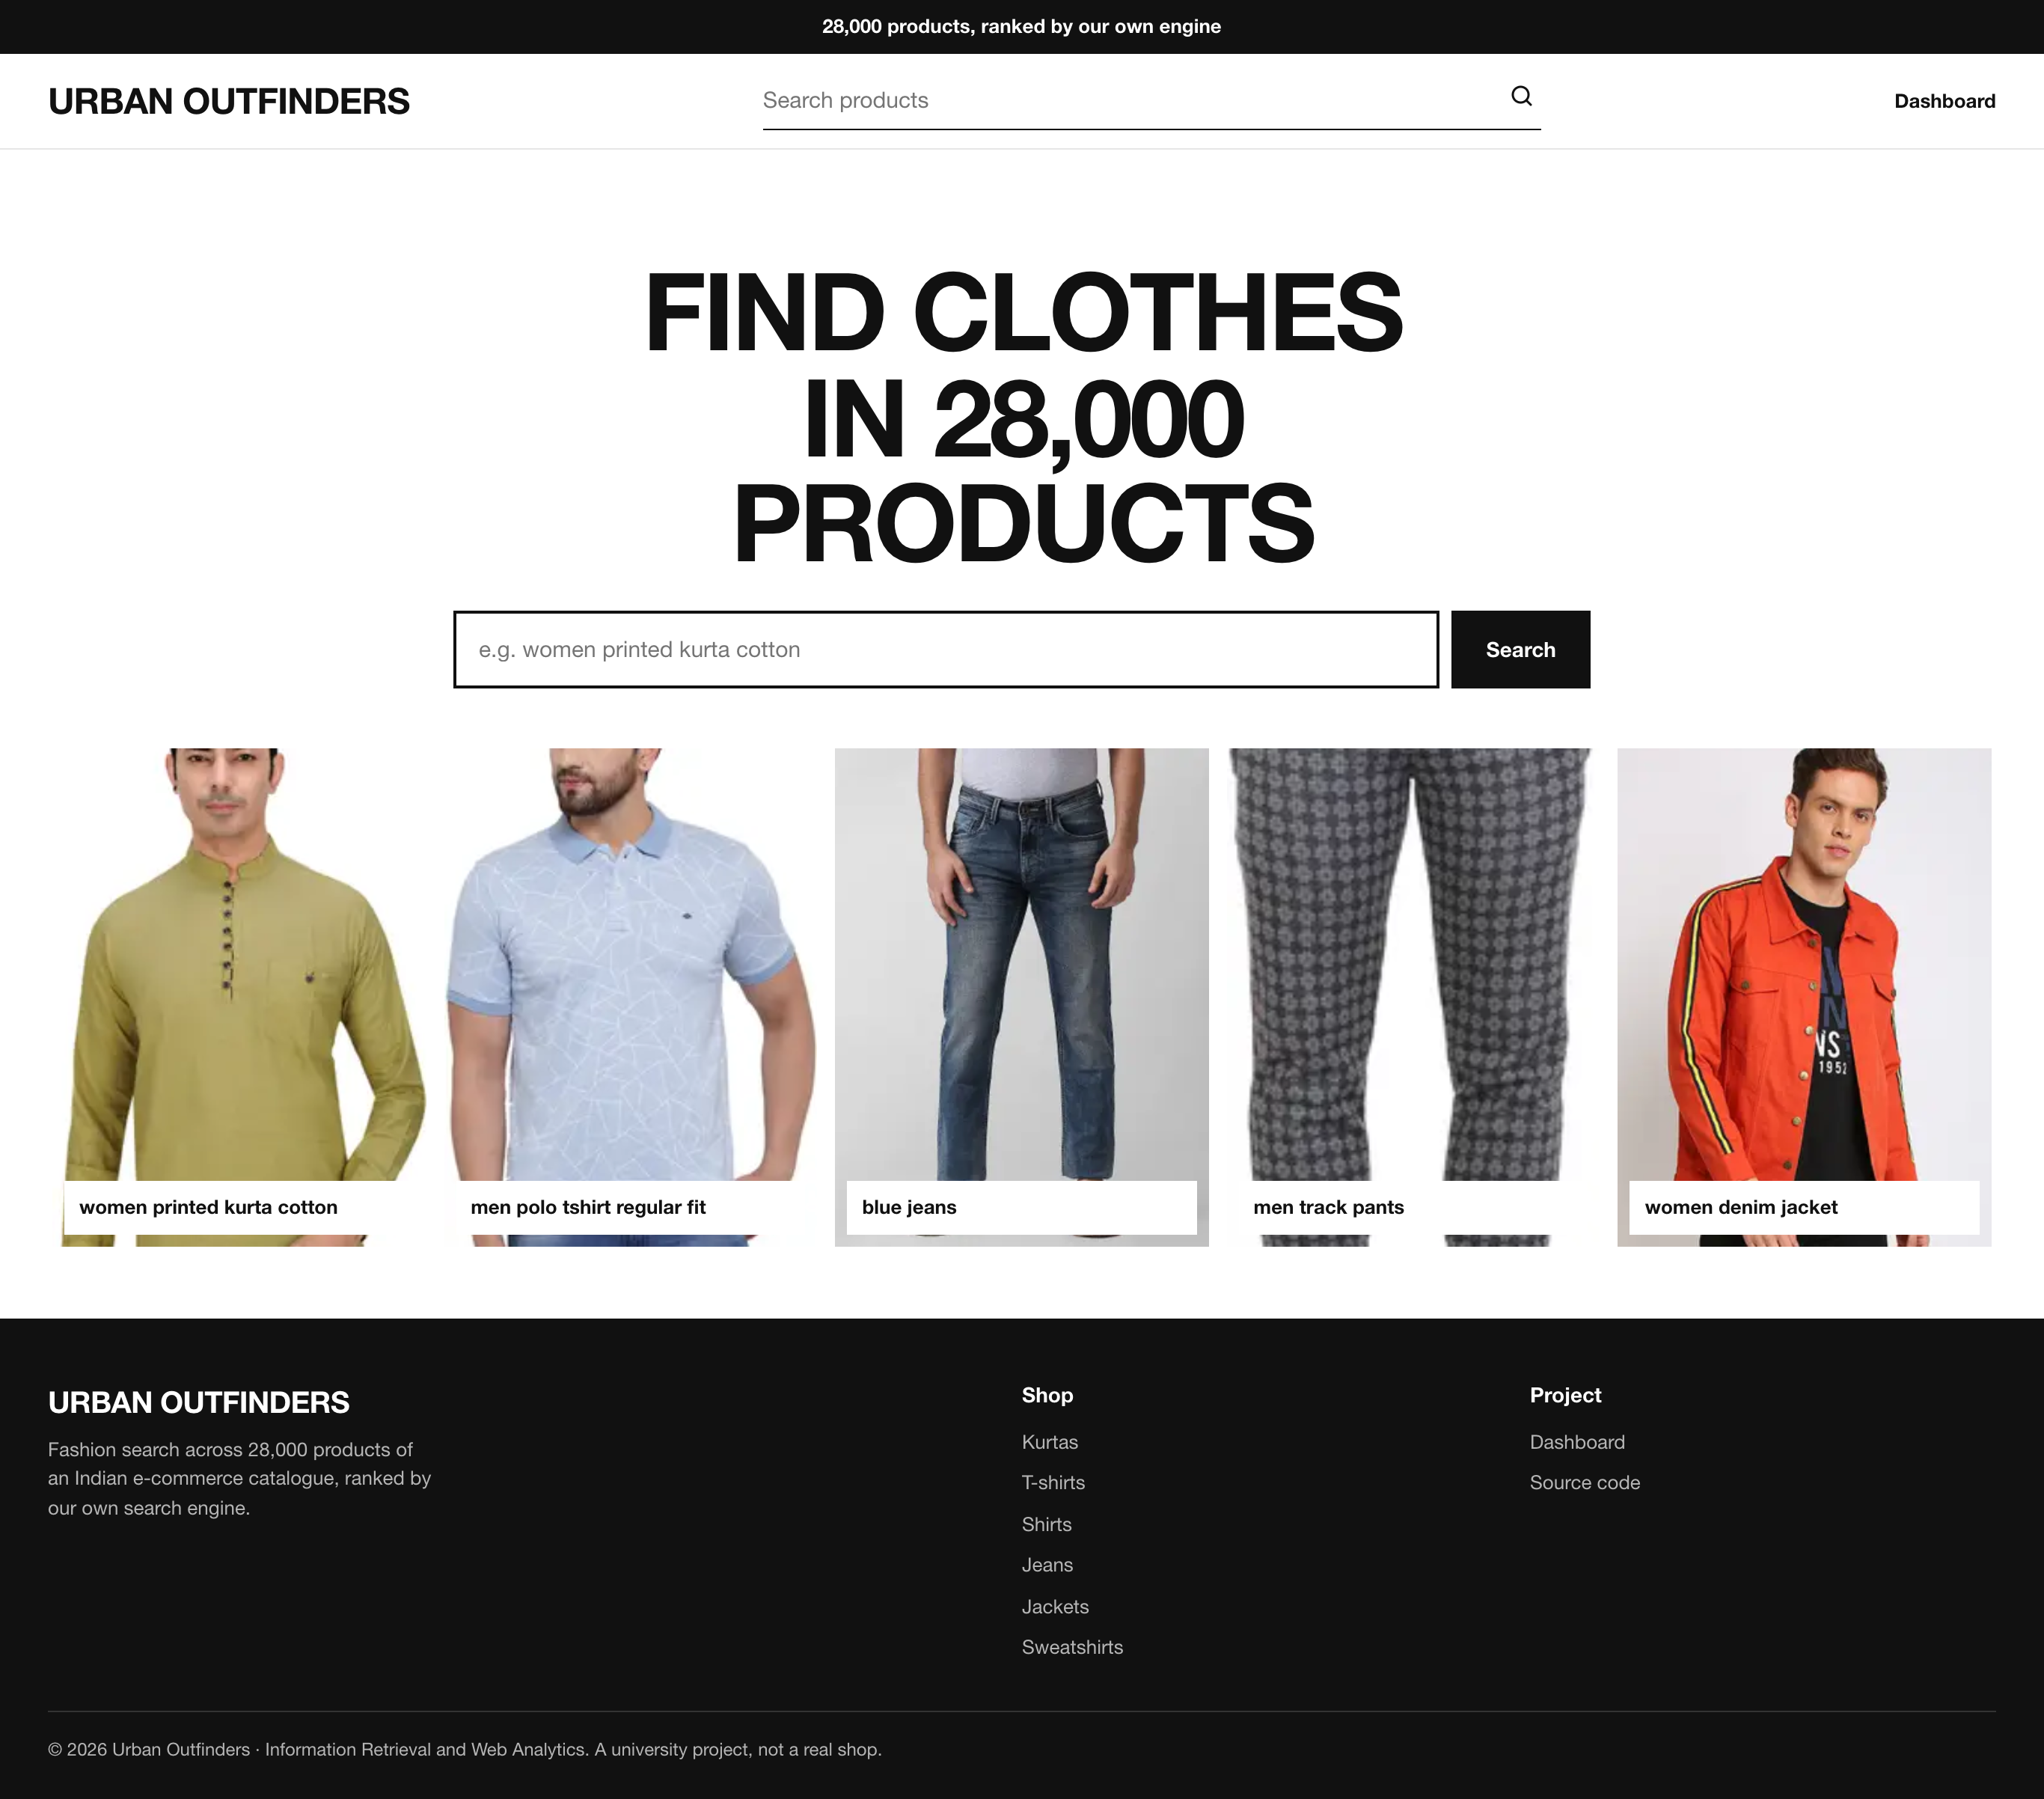
\includegraphics[width=\textwidth]{restyle-home.png}
  \caption{Search page after the visual overhaul, with the footer.}
  \label{fig:restyle-home}
\end{figure}

\begin{figure}[p]
  \centering
  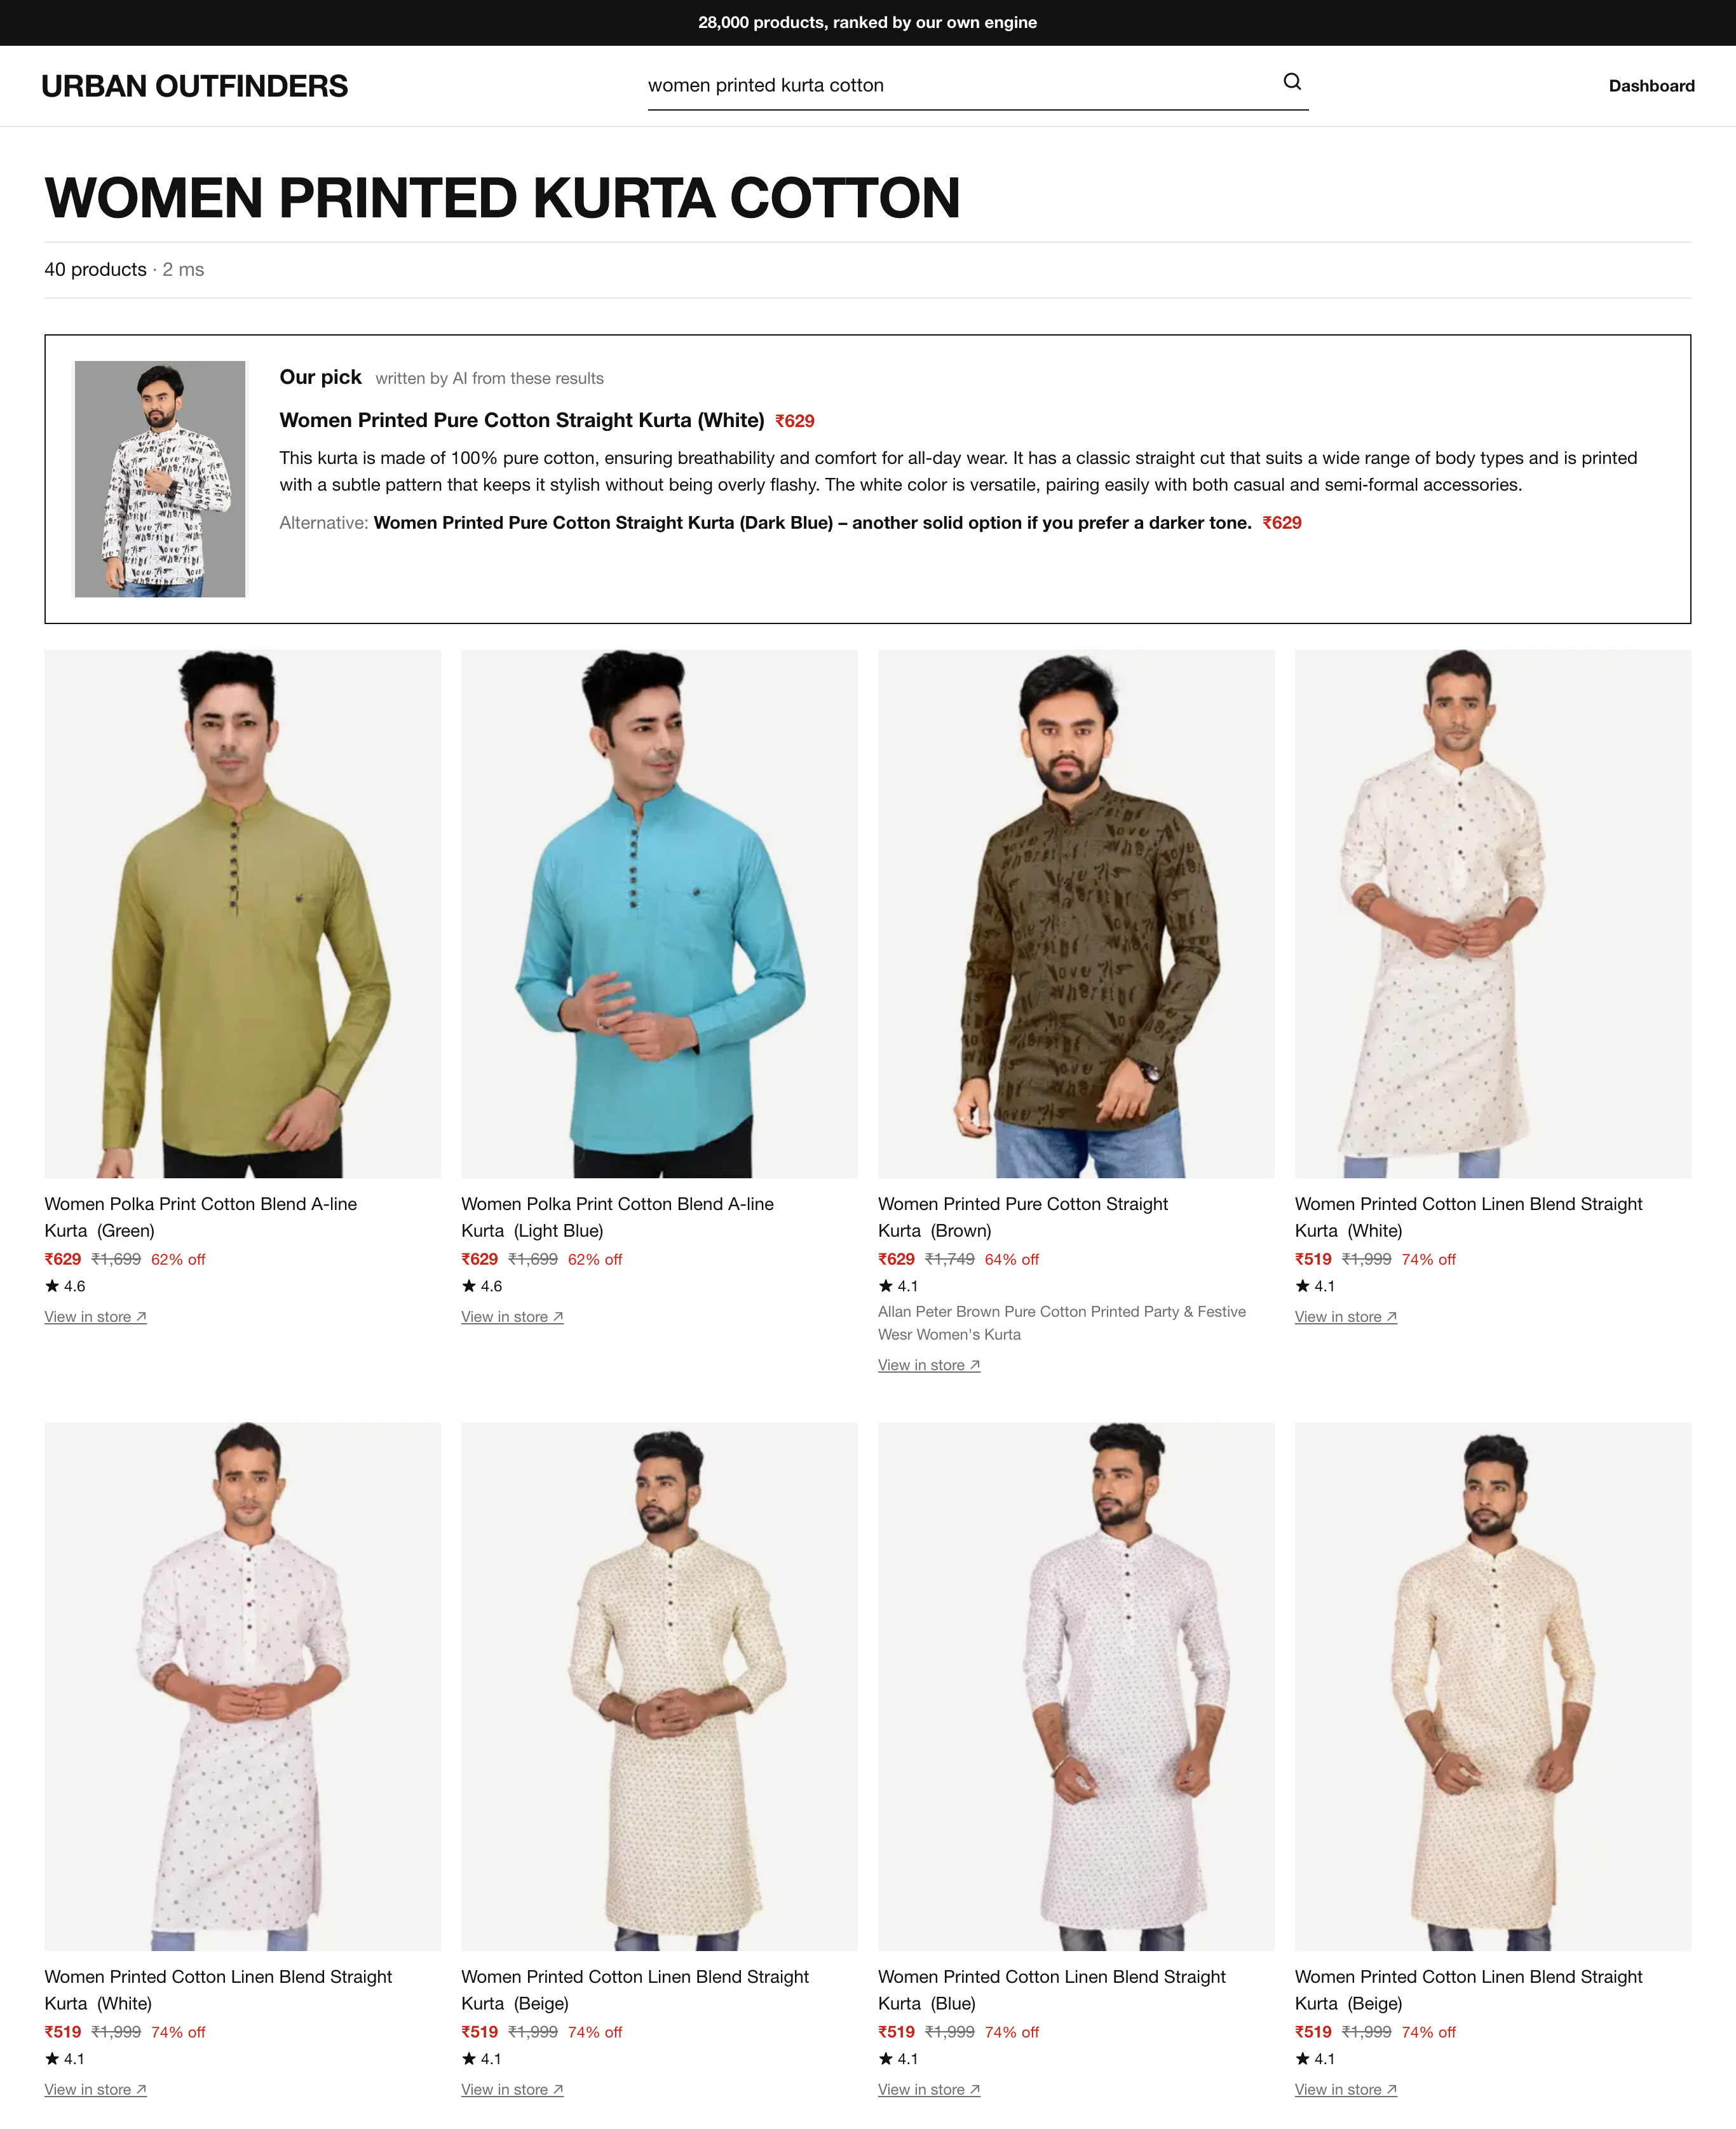
\includegraphics[width=\textwidth]{restyle-results.png}
  \caption{Results page for \emph{women printed kurta cotton}, with the ``Our pick'' card above the products.}
  \label{fig:restyle-results}
\end{figure}

\begin{figure}[p]
  \centering
  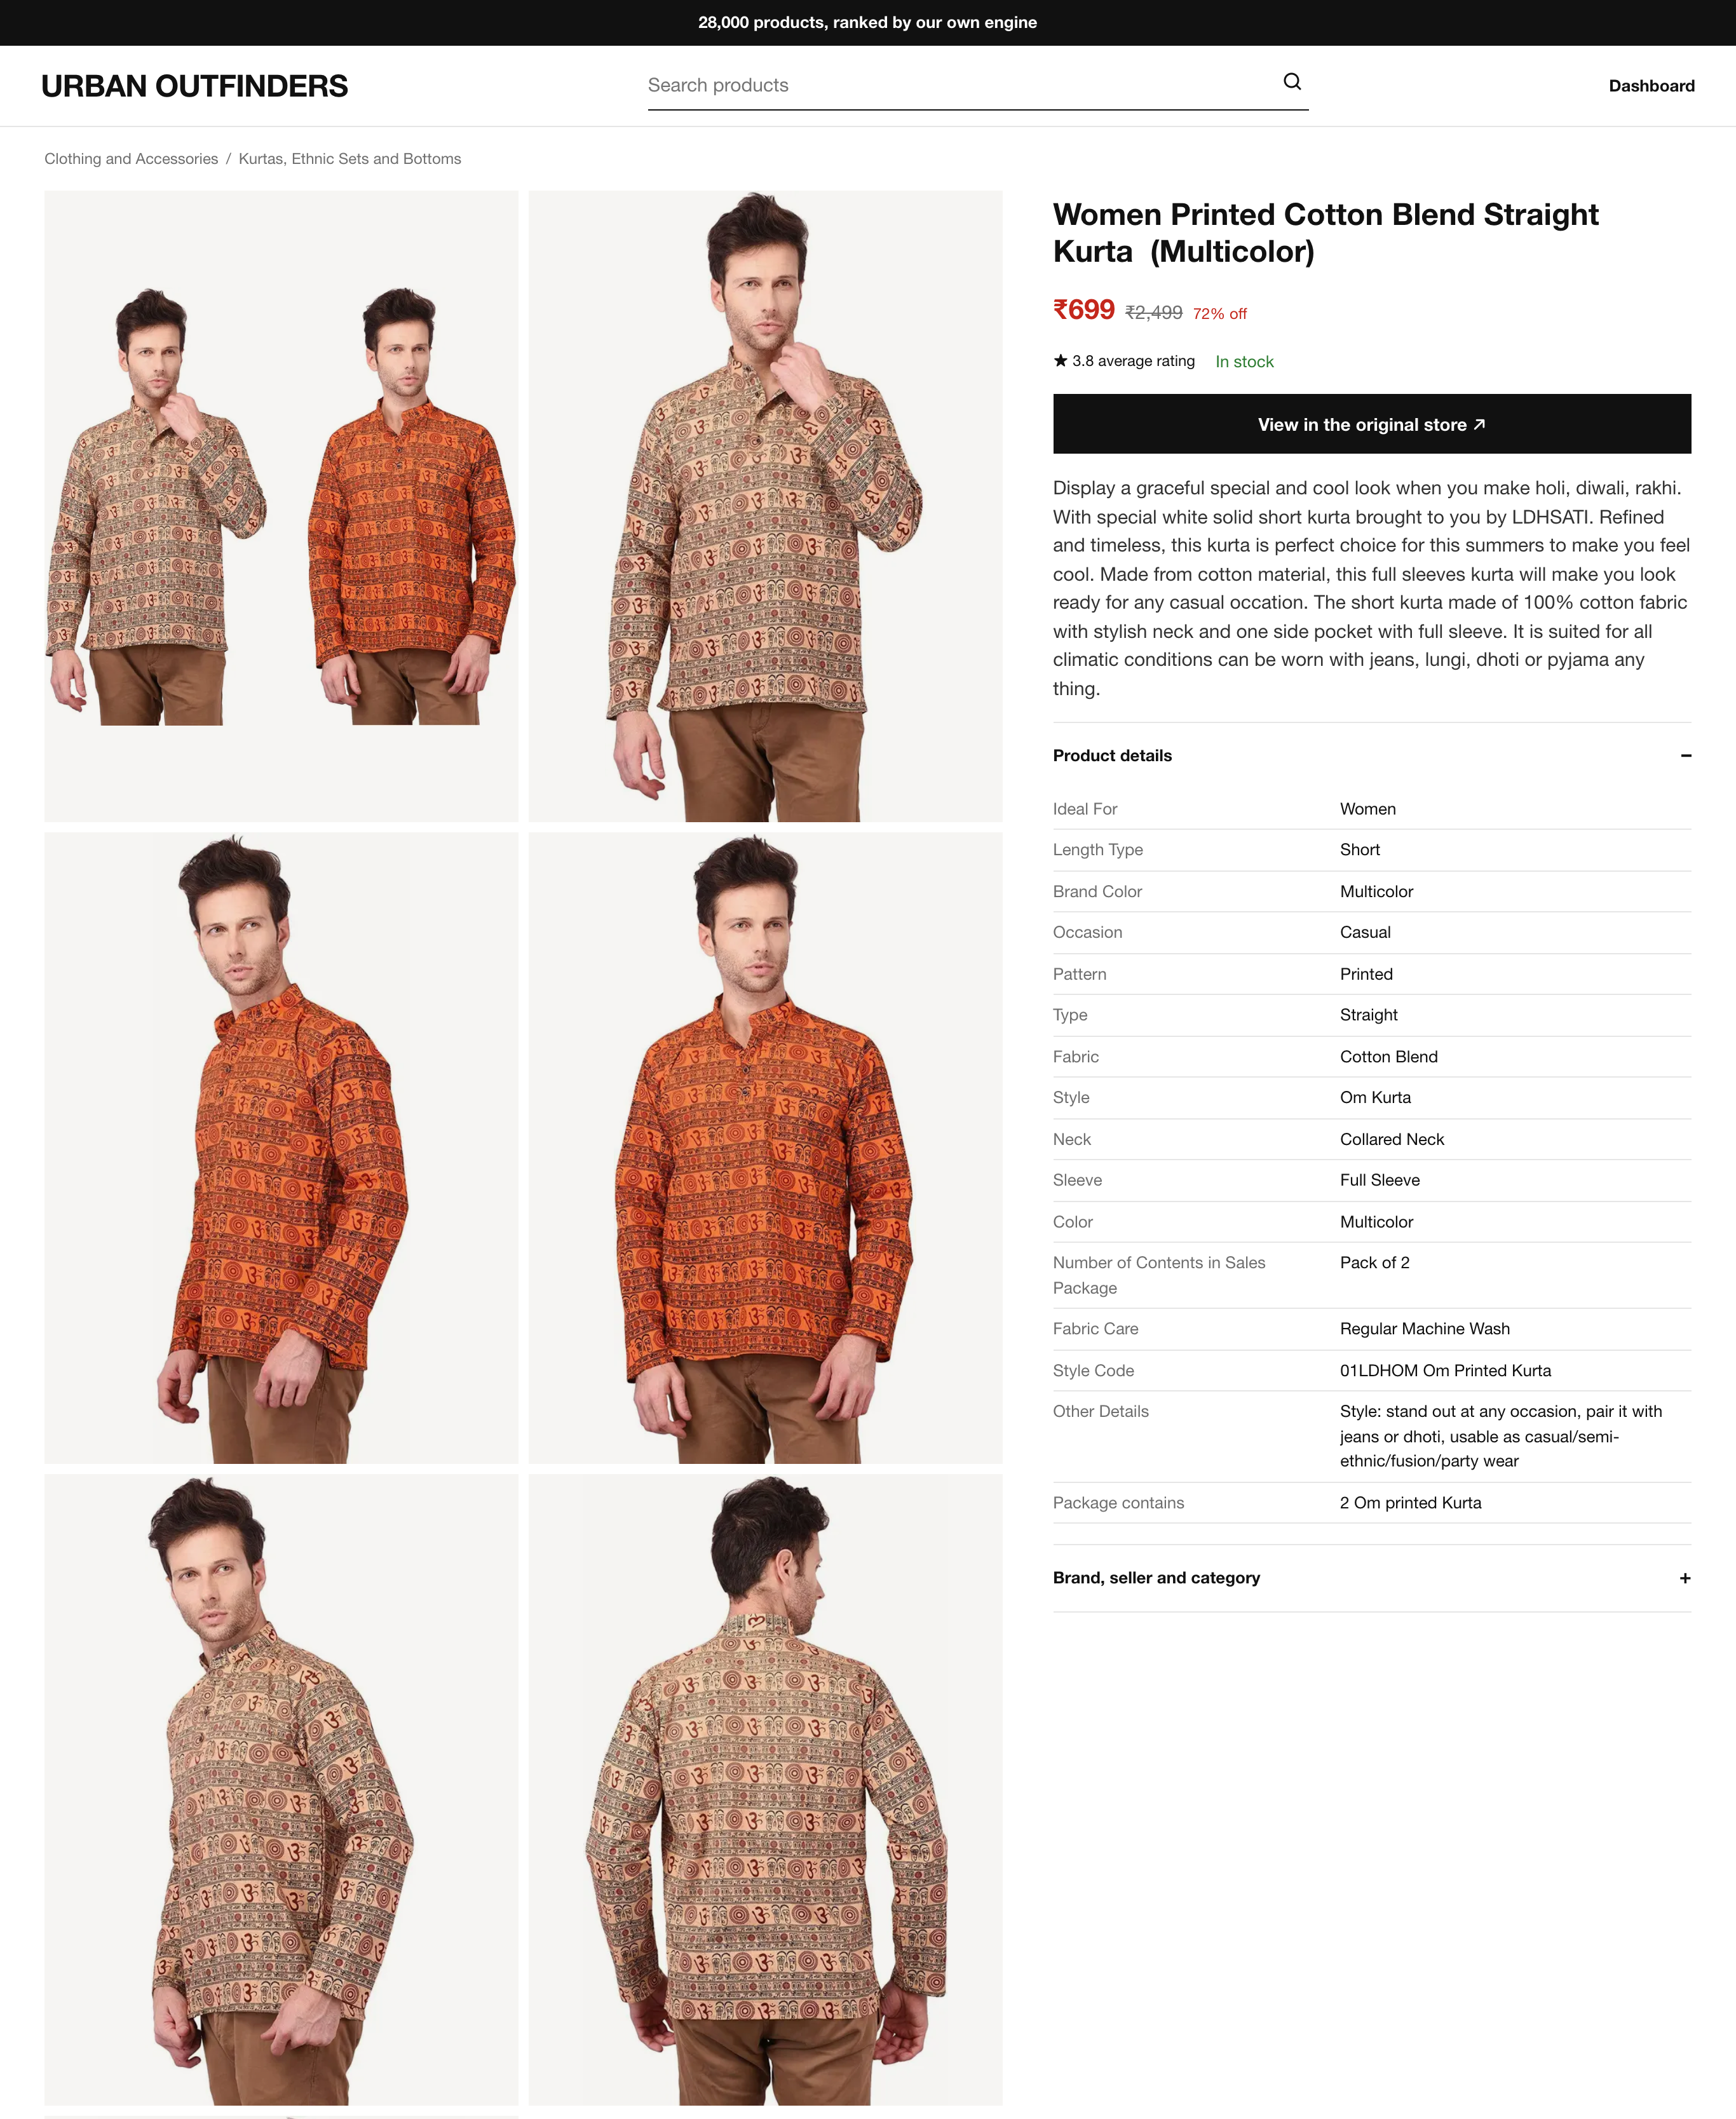
\includegraphics[width=\textwidth]{restyle-product.png}
  \caption{Product page after the visual overhaul (cropped).}
  \label{fig:restyle-product}
\end{figure}

\clearpage
The one feature we removed on purpose is the menu to choose the ranking method. It was useful for this project, to compare the rankers of Part~3 on the same query, but a real shop would never ask its customers to choose a search algorithm. So this version always ranks with the custom score, our best ranker for shopping in Part~3 (the other methods can still be chosen through the URL, for example \texttt{\&method=bm25}). For the same reason, we also removed the line that explained how matching works. The other changes are:
\begin{itemize}
  \item A black strip and a header that stays at the top while scrolling, with the search box on every page, and a dark footer like the ones of commercial sites.
  \item No small labels in capitals above the entries (such as the brand above each product name), which made the pages look busy. The brand is now in the details of the product page.
  \item On the search page, the example queries shown as picture tiles. Hovering a tile hides its label and fades through the pictures of the first results of that query. These are five popular searches that all get an ``Our pick'' (two of the Part~2 test queries, \emph{slim fit jogger men} and \emph{puma men tshirt}, get no recommendation from the baseline prompt, so we replaced them with \emph{blue jeans} and \emph{men track pants}).
  \item Results as a grid of picture cards. Hovering a card fades to the second picture of the product, and keeps rotating through its other pictures while the mouse stays on it.
  \item The LLM summary shown as an ``Our pick'' card, with the picture, name and price of the recommended product and of the alternative, each linked to its page (the app finds the product IDs that the LLM writes among the results). While the summary is being written, the card shows an animated loading placeholder.
  \item On the product page, large pictures in a two-column gallery with the details next to them, and the product details and seller in sections that can be opened and closed.
  \item A mobile-first layout (\cref{fig:restyle-phone}). On a phone, the header search moves below the logo, the cards keep two columns and the product pictures become a carousel to swipe.
\end{itemize}

\begin{figure}[!hb]
  \centering
  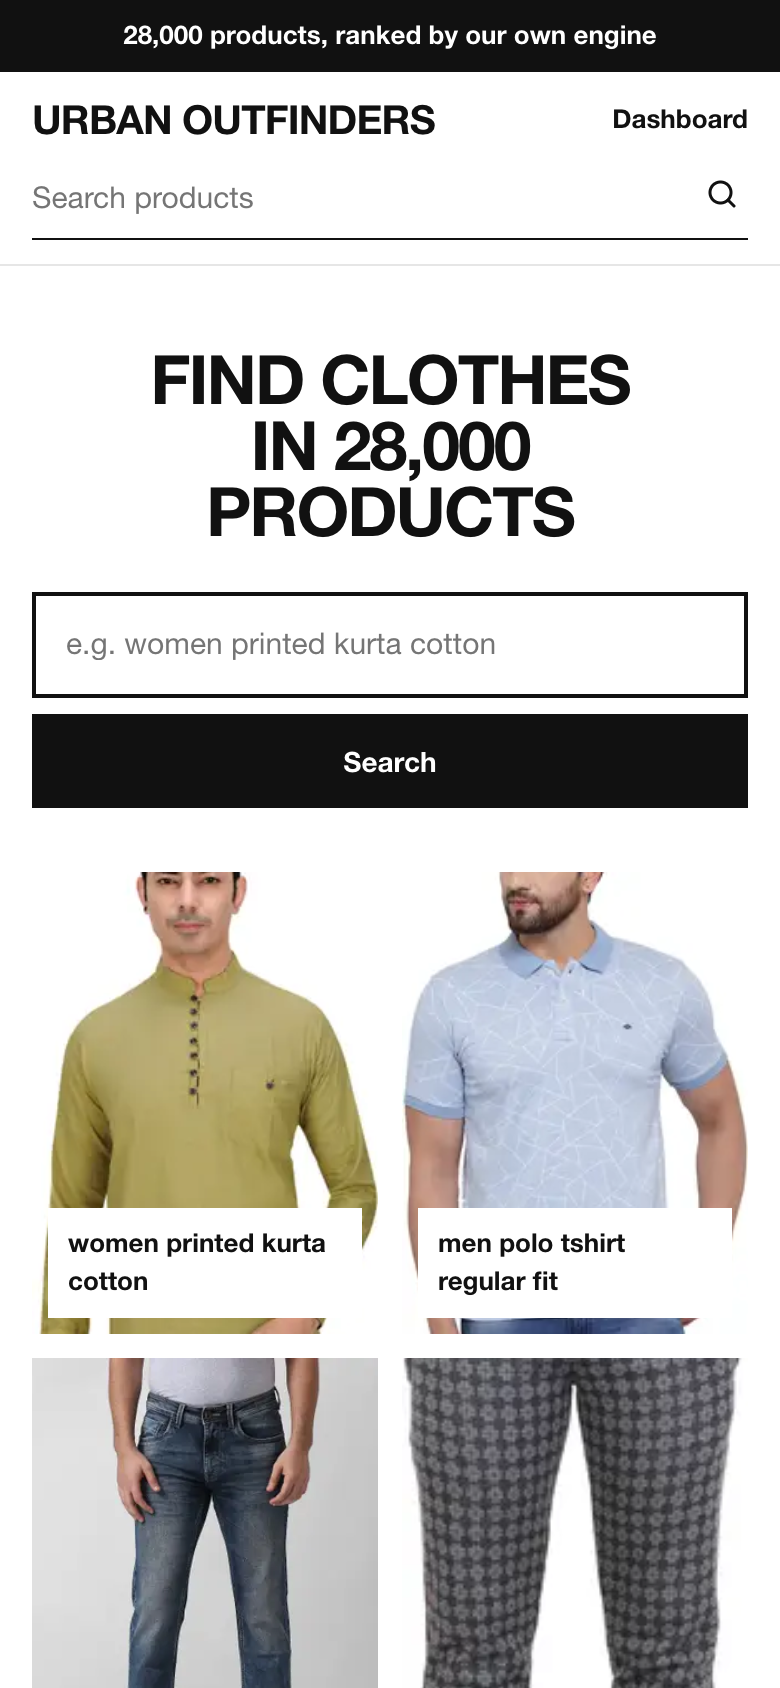
\includegraphics[width=0.24\textwidth]{restyle-phone-home.png}\hfill
  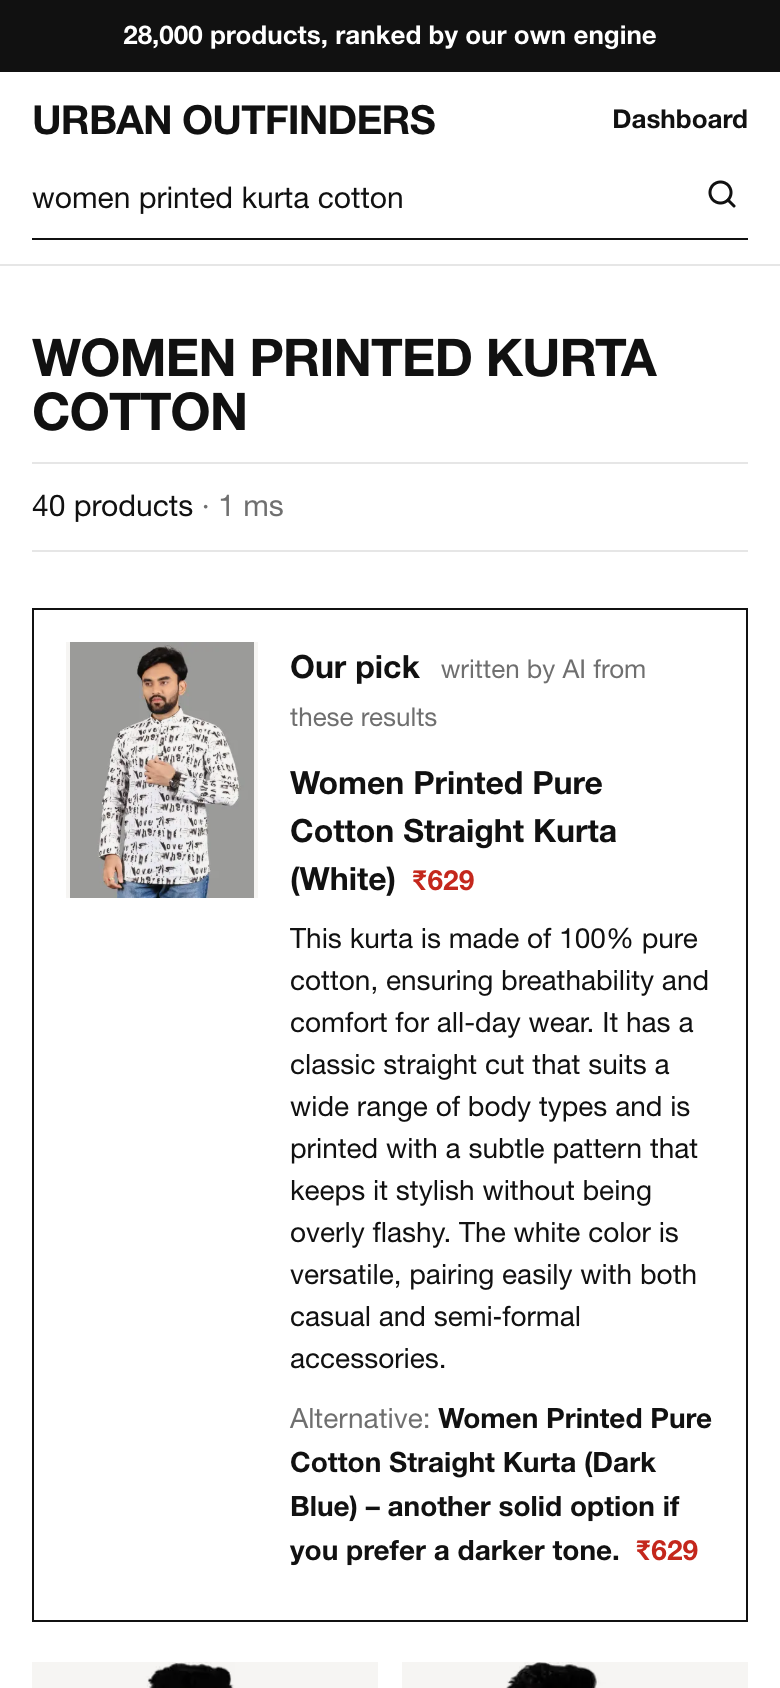
\includegraphics[width=0.24\textwidth]{restyle-phone-results.png}\hfill
  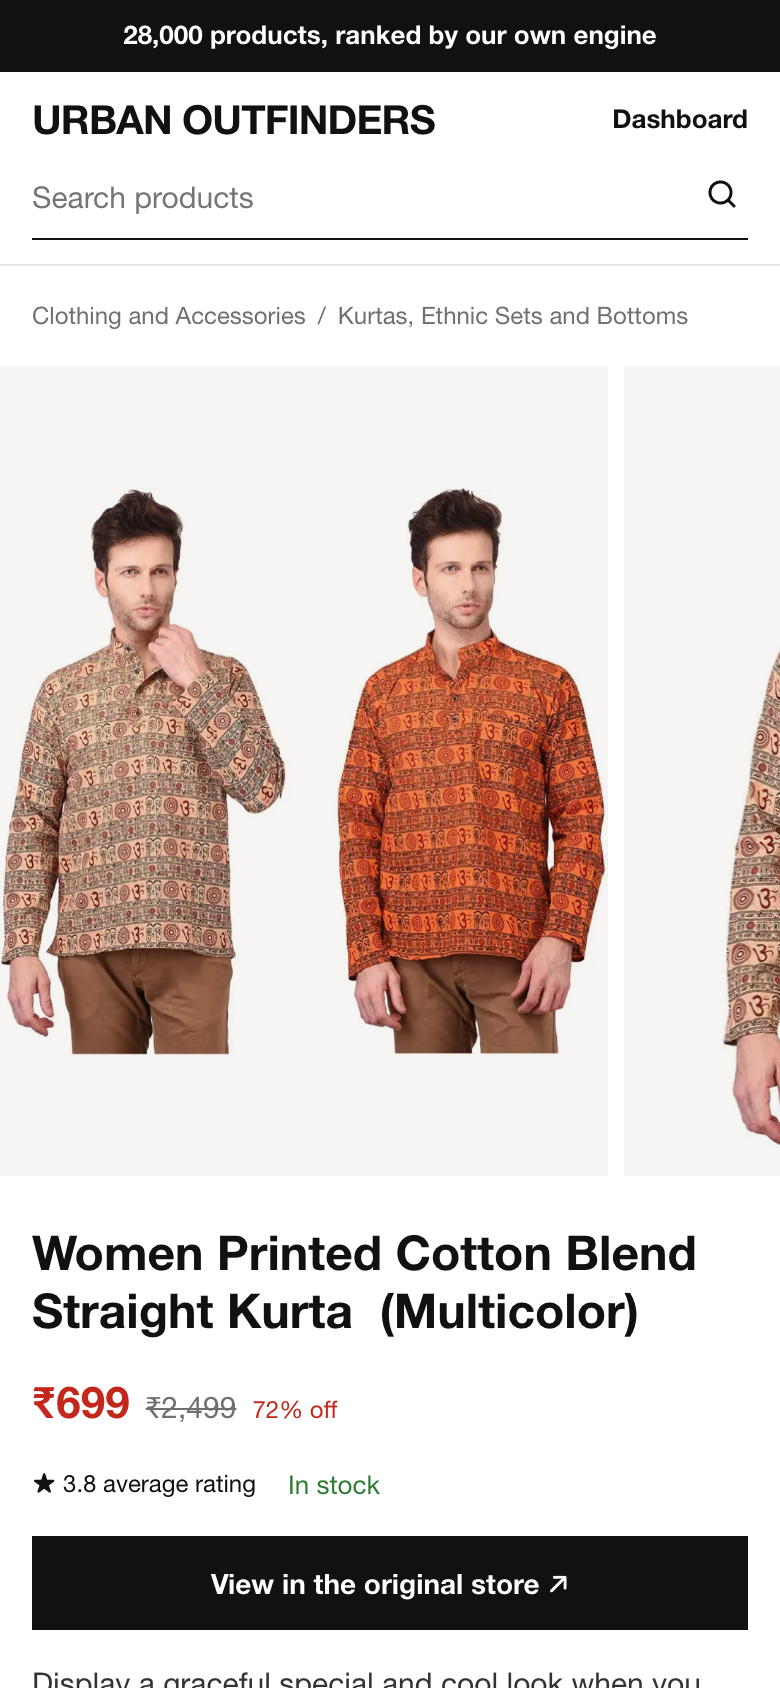
\includegraphics[width=0.24\textwidth]{restyle-phone-product.png}
  \caption{Search, results and product pages on a phone screen (390 pixels wide).}
  \label{fig:restyle-phone}
\end{figure}

\end{document}
